\chapter{Methods}

\emph{CRAX}\autocite{huang2012crax} has been a success on generating
Linux/Windows exploit automatically. \emph{CRAXDroid} leverages the power of
\emph{CRAX} to generate exploit for Android, which is a Linux-based operating
system. To exploit Android, we start digging from the very outer skin---apps.

Apps are mostly written in Java and compiled into bytecode. Apps are then run
by DVM (Dalvik Virtual Machine), which translate bytecode into machine specific
language. Since the translation takes time and bytecode is easily decompiled
into human readable Java code, JNI (Java Native Interface) is introduced in
order to improve performance or to conceal business logic.

To use JNI, app developers first implement the desired program logic in
C/C++/Assembly, and compile the source code into a native shared library. Apps
then load the shared library through System.loadLibrary() method in order to
use it. While JNI extends the power of Android apps, it also increases the
chance that the apps suffer from known vulnerabilities, such as stack overflow,
heap overflow, etc.

To exploit a program basically means to hijack the control flow of a process
via known vulnerabilities. And the hijacking task usually involves PC (program
counter), or referred to IP (instruction pointer) on some architectures,
forging. The PC register stores a memory address, which pointed to a
instruction to be run by the CPU. If the PC register could somehow be affected
by some user controllable input, a hacker might be able to make the CPU execute
customized, and usually malicious, instructions, for example, instructions to
spawn a shell.

\emph{CRAX} uses \emph{S$^{2}$E}\autocite{chipounov2011s2e}, a system analysis
platform based on symbolic execution, to find out how cirtical factors, such as
PC, are related to user controllable input.

\begin{figure}[!ht]
  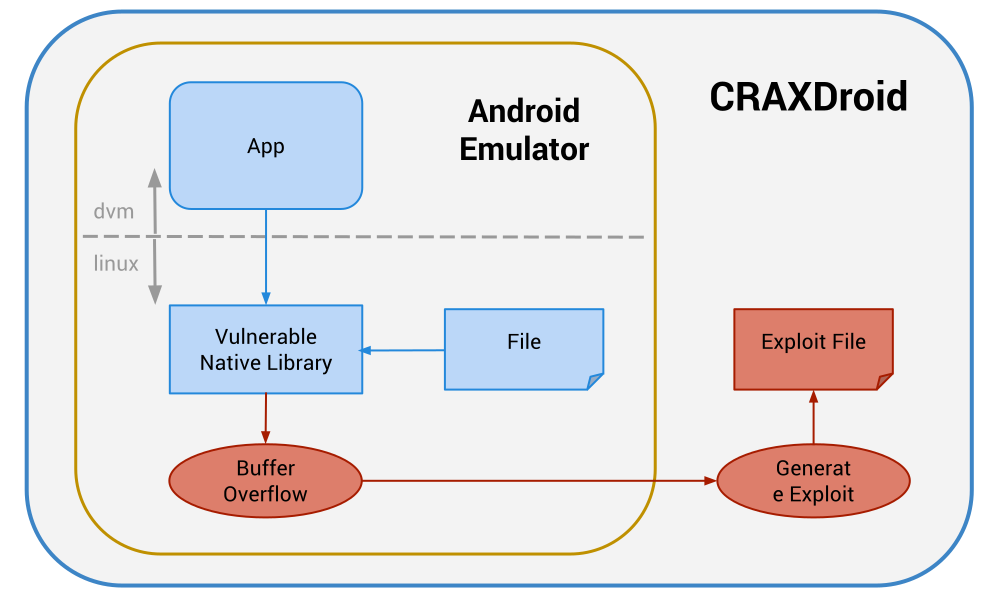
\includegraphics[width=\textwidth]{android-exploit-scenario}
  \caption{An Exploit Scenario on Android}
  \label{fig:android-exploit-scenario}
\end{figure}
